\documentclass[10pt]{beamer}

\usepackage{tikz}
\usetikzlibrary{positioning,shapes,shadows,arrows}
\tikzstyle{abstract}=[rectangle, rounded corners, draw=black, anchor=north, fill=blue!10, text centered, minimum height={height("Gp")+2pt}, minimum width=3cm, font=\footnotesize]

\definecolor{links}{HTML}{0000CC}
\hypersetup{colorlinks,linkcolor=,urlcolor=links}

\mode<handout>
{
  \usepackage{pgfpages}
  \pgfpagesuselayout{4 on 1}[a4paper,border shrink=3mm,landscape]
  \usetheme{CambridgeUS}
  \usecolortheme{lily}
}

\mode<beamer>
{
  \usetheme{CambridgeUS}
}

\AtBeginSection[]
{
  \begin{frame}
    \frametitle{Outline}
    \tableofcontents[currentsection]
  \end{frame}
}

\setbeamerfont{frametitle}{family=\rmfamily,series=\bfseries,size={\fontsize{10}{10}}}
\setbeamertemplate{frametitle continuation}[from second]

\title{Dynare Time Series \& Reporting}
\author{Houtan Bastani}
\institute{CEPREMAP}
\date{13 June 2014}

\begin{document}

\begin{frame}
  \titlepage
\end{frame}

\begin{frame}[t]
  \frametitle{Outline}
  \tableofcontents
\end{frame}

%
% DATES
%
\section{Time Series}

\subsection{Overview}
\begin{frame}[fragile,t]
  \frametitle{Overview}
  \begin{itemize}
  \item Provide support for time series in Dynare
  \item Introduced in Dynare 4.4
  \item Currently only used for reporting.
  \item Use will increase with time (\textit{e.g.,} to be included in new estimation code)
  \end{itemize}
\end{frame}


\subsection{Syntax}
\begin{frame}[fragile,t]
  \frametitle{Syntax}
  \begin{itemize}
  \item Two components of a time series:
    \begin{itemize}
    \item A time component. In Dynare: \texttt{dates}
    \item A data component mapped to time. In Dynare: \texttt{dseries}
    \end{itemize}
  \end{itemize}
\end{frame}

\subsubsection{\texttt{dates} Syntax}
\begin{frame}[fragile,t]
  \frametitle{\texttt{dates} Syntax}
  \begin{itemize}
  \item The \texttt{dates} command creates an object that represents at least one date at a given frequency
    \begin{itemize}
    \item Yearly: \texttt{`Y', `y', 1}
    \item Quarterly: \texttt{`Q', `q', 4}
    \item Monthly: \texttt{`M', `m', 12}
    \item Weekly: \texttt{`W', `w', 52}
    \end{itemize}
  \item It has two slightly different syntaxes
    \begin{itemize}
    \item One for inclusion in \texttt{.m} files
    \item One for inclusion in \texttt{.mod} files (simplified using the preprocessor)
      \begin{itemize}
        \item To prevent date translation, escape the date with `\texttt{\$}' (\textit{e.g.,} \texttt{\$2020y})
      \end{itemize}
    \end{itemize}
  \item Minimal restrictions on dates. Can be
    \begin{itemize}
      \item Negative
      \item Empty
      \item Noncontiguous
    \end{itemize}
  \end{itemize}
\end{frame}


\begin{frame}[fragile,t]
  \frametitle{Creating a new \texttt{dates} object}
  \begin{itemize}
  \item A single date:
    \begin{itemize}
    \item In a \texttt{.m} file: \texttt{t = dates(`1999y');}
    \item In a \texttt{.mod} file: \texttt{t = 1999y;}
    \end{itemize}
  \item A date range:
    \begin{itemize}
    \item In a \texttt{.m} file: \texttt{dr = dates(`1999y'):dates(`2020y');}
    \item In a \texttt{.mod} file: \texttt{dr = 1999y:2020y;}
    \end{itemize}
  \end{itemize}
\end{frame}


\begin{frame}[fragile,t]
  \frametitle{Modifying \texttt{dates}}
  \begin{itemize}
  \item \texttt{append}: appends a date to the date
    \begin{itemize}
    \item \texttt{t=t.append(dates(`1900y')); \% <dates: 1999Y, 1900Y>}
    \end{itemize}
  \item \texttt{horzcat}: horizontal concatenation
    \begin{itemize}
    \item \texttt{[t t]; \% <dates: 1999Y, 1900Y, 1999Y, 1900Y>};
    \end{itemize}
  \item \texttt{minus}: either the distance between two \texttt{dates} or lag one \texttt{dates}
    \begin{itemize}
    \item \texttt{t-t \% [0 0]'}
    \item \texttt{t-[3 3]' \% <dates: 1996Y, 1897Y>}
    \end{itemize}
  \item \texttt{plus}: either combine two \texttt{dates} or forward one \texttt{dates}
    \begin{itemize}
    \item \texttt{t+t \% <dates: 1999Y, 1900Y, 1999Y, 1900Y>}
    \item \texttt{t+[3 3]' \% <dates: 2002Y, 1903Y>}
    \end{itemize}
  \item \texttt{pop}: remove last element
    \begin{itemize}
    \item \texttt{t.pop(); \% <dates: 1999Y>}
    \end{itemize}
  \item \texttt{sort}: sort dates in ascending order
    \begin{itemize}
    \item \texttt{t=t.sort(); \% <dates: 1900Y, 1999Y>}
    \end{itemize}
  \item \texttt{uminus}: shifts dates back one period
    \begin{itemize}
    \item \texttt{-t; \% <dates: 1998Y, 1899Y>}
    \end{itemize}
  \item \texttt{unique}: removes repetitions
    \begin{itemize}
    \item \texttt{t.append(dates(`1999y')).unique() \% <dates: 1900Y, 1999Y>}
    \end{itemize}
  \item \texttt{uplus}: shifts dates forward one period
    \begin{itemize}
    \item \texttt{++t; \% <dates: 2001Y, 1902Y>}
    \end{itemize}
  \end{itemize}
\end{frame}


\begin{frame}[fragile,t]
  \frametitle{Getting info about \texttt{dates}}
  \begin{itemize}
  \item \texttt{char}: returns a single date as a string
    \begin{itemize}
    \item \texttt{t(1).char() \% 1999Y}
    \end{itemize}
  \item \texttt{double}: returns a floating point representation of the date
    \begin{itemize}
    \item \texttt{t.double() \% [1999 1900]'}
    \end{itemize}
  \item \texttt{freq}: returns the frequency
    \begin{itemize}
    \item \texttt{t.freq; \% 1}
    \end{itemize}
  \item \texttt{isequal}: returns true if the two arguments are equal
    \begin{itemize}
    \item \texttt{isequal(t,t) \% 1}
    \end{itemize}
  \item \texttt{length}: returns the number of dates
    \begin{itemize}
    \item \texttt{t.length() \% 2}
    \end{itemize}
  \item \texttt{max}: returns the maximum \texttt{dates} in the arguments
    \begin{itemize}
    \item \texttt{max(t,dr) \% <dates: 2020Y>}
    \end{itemize}
  \item \texttt{min}: returns the minimum \texttt{dates} in the arguments
    \begin{itemize}
    \item \texttt{min(t,dr) \% <dates: 1900Y>}
    \end{itemize}
  \item \texttt{eq, ge, gt, le, lt, ne}: returns boolean value of comparison
    \begin{itemize}
    \item \texttt{t==t \% [1 1]'}
    \item \texttt{t>=dates(`1950y') \% [1 0]'}
    \item \texttt{t$\thicksim$=dates(`1999y') \% [0 1]'}
    \end{itemize}
  \end{itemize}
\end{frame}

\begin{frame}[fragile,t]
  \frametitle{Set Operations on \texttt{dates}}
  \begin{itemize}
  \item \texttt{intersect}: returns the intersection of the arguments
    \begin{itemize}
    \item \texttt{intersect(t,dr) \% <dates: 1999Y>}
    \end{itemize}
  \item \texttt{isempty}: returns true if the argument is empty
    \begin{itemize}
    \item \texttt{isempty(t) \% 0}
    \end{itemize}
  \item \texttt{setdiff}: returns dates present in first arg but not in second
    \begin{itemize}
    \item \texttt{setdiff(t,dr) \% <dates: 1900Y>}
    \end{itemize}
  \item \texttt{union}:
    \begin{itemize}
    \item \texttt{union(dr,t) \% <dates: 1900Y, 1999Y,  ..., 2019Y, 2020Y>}
    \end{itemize}
  \end{itemize}
\end{frame}


%
% DSERIES
%
\subsubsection{\texttt{dseries} Syntax}


\subsection{Examples}


%
% REPORTING
%
\section{Reporting}
\subsection{Overview}
\begin{frame}
  \frametitle{Overview}
  \begin{itemize}
  \item Introduced in Dynare 4.4
  \item Introduce reporting functionality to Dynare
      \begin{itemize}
      \item Input: \texttt{dseries}
      \item Output: \LaTeX\ report \& compiled \texttt{.pdf}
      \end{itemize}
    \item Graphs and Tables are modular
      \begin{itemize}
      \item Can easily be included in another document
      \end{itemize}
    \item Graphs are produced in Ti$k$Z
      \begin{itemize}
      \item Scales well
      \item Formating follows that of enclosing document
      \end{itemize}
    \item Works with Matlab \& Octave
    \item Works approximately 5 times faster than Iris reporting
  \end{itemize}
\end{frame}

\begin{frame}
  \frametitle{Reporting Class Hierarchy}
  \centering {
    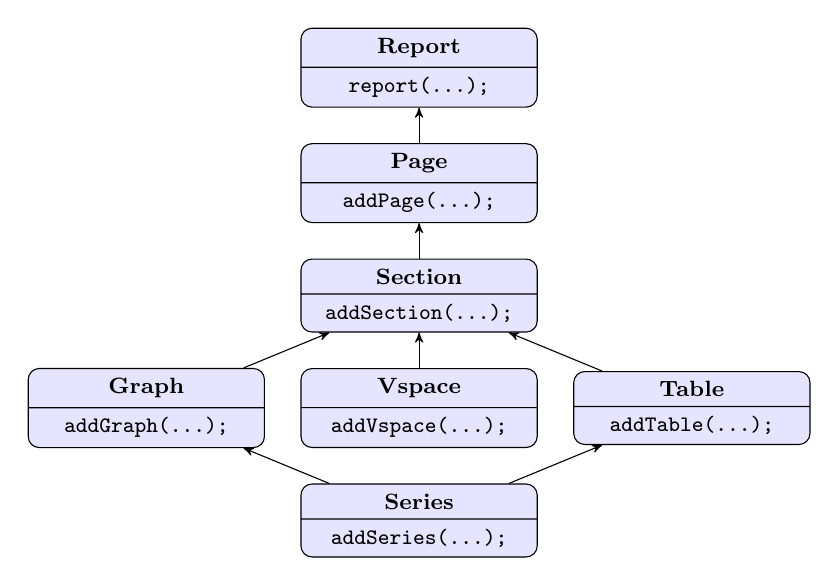
\begin{tikzpicture}[
        node distance = .45cm,
        auto,
        line/.style={->, >=stealth'},
      ]
      \node (Report) [abstract, rectangle split, rectangle split parts=2]
            {
              \textbf{Report}
              \nodepart{second}\texttt{report(...);}
            };
      \node (Page) [abstract, rectangle split, rectangle split parts=2, below=of Report]
            {
              \textbf{Page}
              \nodepart{second}\texttt{addPage(...);}
            };
      \node (Section) [abstract, rectangle split, rectangle split parts=2, below=of Page]
            {
              \textbf{Section}
              \nodepart{second}\texttt{addSection(...);}
            };
      \node (Vspace) [abstract, rectangle split, rectangle split parts=2, below=of Section]
            {
              \textbf{Vspace}
              \nodepart{second}\texttt{addVspace(...);}
            };
      \node (Graph) [abstract, rectangle split, rectangle split parts=2, left=of Vspace]
            {
              \textbf{Graph}
              \nodepart{second}\texttt{addGraph(...);}
            };
      \node (Table) [abstract, rectangle split, rectangle split parts=2, right=of Vspace, text height=]
            {
              \textbf{Table}
              \nodepart{second}\texttt{addTable(...);}
            };
      \node (Series) [abstract, rectangle split, rectangle split parts=2, below=of Vspace]
            {
              \textbf{Series}
              \nodepart{second}\texttt{addSeries(...);}
            };
      \draw [line] (Series) to node { } (Table);
      \draw [line] (Series) to node { } (Graph);
      \draw [line] (Table) to node { } (Section);
      \draw [line] (Graph) to node { } (Section);
      \draw [line] (Vspace) to node { } (Section);
      \draw [line] (Section) to node { } (Page);
      \draw [line] (Page) to node { } (Report);
    \end{tikzpicture}
  }
\end{frame}

\subsection{Syntax}


\subsection{Examples}

\end{document}
